
    \section{Quantum Complexity}
    \subsection{Quantum Mechanics}
    \setbeamercovered{invisible}
    \begin{frame}{Schrodinger's cat}
        \begin{columns}[onlytextwidth]
            \column{0.5\textwidth}
            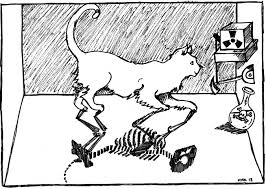
\includegraphics[width=\linewidth]{images/cat.jpg}
        \column{0.5\textwidth}
        \begin{itemize}
            \item Assume there is a cat in a box, with a handle 
            that will break the poison bottle based on the reaction of a quantum particle
            \pause
            \item Is the cat dead or alive?
            \pause
            \item Neither, the cat is bound to the \alert{SuperPosition} of the
            quantum particle, being both dead and alive at the same time.
        \end{itemize}
        
        \end{columns}
    \end{frame}
    \setbeamercovered{transparent}
    \begin{frame}{Why measurement alters the state}
        \begin{itemize}
            \item Niels Bohr  (Copenhagen interpretation):\\
            In essence this interpretation amounts to a sophisticated way of saying not to ask the question. Science relies on the notion of measurements and observations, so in essence asking in quantum mechanics “what is a measurement?” is equivalent to asking the axioms of euclidean geometry “what is a point?”.
        \end{itemize}
    \end{frame}
    \begin{frame}{Why measurement alters the state}
        \begin{itemize}
            \item Hugh Everett  (Many worlds interpretation):\\
            There is only one process in quantum mechanics, unitary evolution. What we perceive as measurements is just unitary evolution applied to the measuring equipment and the observer. Essentially the universe splits every time a measurement is performed, and one copy sees $|0\rangle$ while the other sees $|1\rangle$.            
        \end{itemize}
    \end{frame}
    \begin{frame}{Why measurement alters the state}
        \begin{itemize}
        
            \item David Bohm  (Non-local hidden variables):\\
            The third answer says that both of the previous answers are unacceptable, so quantum mechanics is somehow incomplete in the sense that there is an additional aspect that we’re missing. Non-local hidden variables is one proposal to fill that gap, but there are others.
        \end{itemize}
    \end{frame}
    \subsection{Quantum Computing}
    
    \begin{frame}{Qubits and data representation}
        \begin{itemize}
            \item We represent Superposition of data with a vector in complex space with a length of 1.
            \item We represent the value of the vector with the unit basis of our space.
            \item For the purpose of this lecture we follow the traditional representation by Qubits:
                \begin{itemize}
                    \item We represent one qubit with $|x\rangle $ with definition:\\
                    $|0\rangle := \begin{bmatrix}
                        1\\
                        0
                    \end{bmatrix}$
                    $|1\rangle := \begin{bmatrix}
                        0\\
                        1
                    \end{bmatrix}$
                    \item We define n not \alert{entangled} qubit with this notation:\\
                    $|x\rangle^{\oplus n} := \underbrace{|x\rangle|x\rangle \dots |x\rangle}_n $
                \end{itemize}
        \end{itemize}
    \end{frame}
    \begin{frame}{Qubits and data representation}
        \begin{itemize}
            \item Similarly we represent n \alert{entangled} multi-qubits with n basis vectors\\
            $|00\rangle := \begin{bmatrix}
                1\\
                0\\
                0\\
                0
            \end{bmatrix}$
            $|01\rangle := \begin{bmatrix}
                0\\
                1\\
                0\\
                0
            \end{bmatrix}$
            $|10\rangle := \begin{bmatrix}
                0\\
                0\\
                1\\
                0
            \end{bmatrix}$
            $|11\rangle := \begin{bmatrix}
                0\\
                0\\
                0\\
                1
            \end{bmatrix}$
        \end{itemize}
    \end{frame}

    \begin{frame}{Quantum Operations}
        Let us give an example of what a quantum operation looks like.
        We represent quantum operations by multiplying our data by an L2-norm preserving matrix e.g unitary matrices\\
        For example an elementary operation is controlled-NOT (CNOT) that is:\\
        \begin{center}
        $\begin{bmatrix}
            1&0&0&0\\
            0&1&0&0\\
            0&0&0&1\\
            0&0&1&0\\
        \end{bmatrix}$\\
    \end{center}
    it maps $|00\rangle \rightarrow |00\rangle$ , $|01\rangle \rightarrow |01\rangle$
    $|10\rangle \rightarrow |11\rangle$, $|11\rangle \rightarrow |10\rangle$. in other language
    it performs not on the second bit iff the first bit is true or it maps $|xy\rangle \rightarrow |x(x\oplus y)\rangle$

    \end{frame}
    
    % \begin{frame}[plain]{Plain frame}
    \begin{frame}{Measurement}
        We can measure our quantum state by projecting our quantum state vector onto 
        one of our \emph{Orthonormal Basis}. The probability of successful projection is equal to Coefficient power 2.
        for example in our data representation the matrix\\
        \begin{align*}
        \begin{bmatrix}
            \frac{1}{\sqrt{3}}\\
            \sqrt{\frac{2}{3}}
        \end{bmatrix}
        = \frac{1}{\sqrt{3}} |0\rangle + \sqrt{\frac{2}{3}} |1\rangle
    \end{align*}
    So when we measure we get $|0\rangle$ with the probability of 
    $\frac{1}{3}$ and we get $|1\rangle$ with probability of $\frac{2}{3}$.
    \end{frame}
    \begin{frame}{Measurement}
        \begin{block}{Quantum state}
            A quantum state is a n-dimensional complex vector with the length of 1. 
        \end{block}
        \pause
        \begin{block}{Quantum basis state}
            Quantum basis states are a collection of \textbf{Orthonormal basis}
            which we can measure our quantum state with them.
        \end{block}
        \pause
        \begin{block}{Measurement}
            Assume we have a multi-qubit like:\\
            $|a_1a_2 \dots a_n \rangle$ where 
            $\sum_{n = 1}^{n} a_i^2 = 1$
            we can measure this qubit in basis states where the probability
            of us measuring this qubit onto $ith$ state is $a_i^2$
        \end{block}
    \end{frame}
    \begin{frame}{Measurement}
        \begin{exampleblock}{example}
            Assume we can perform a quantum operation which rotates our quantum state
            by $45^o$ the matrix resembling this operation is as follows
            $ \frac{1}{\sqrt{2}}
            \begin{bmatrix}
                1&1\\
                -1&1
            \end{bmatrix}$
            performing this operation twice is equivalent to the NOT operation:\\
            \begin{align*}
                |x\rangle \rightarrow 
                \frac{1}{\sqrt{2}}
                    \begin{bmatrix}
                        1\\
                        -1
                    \end{bmatrix}
                    \rightarrow |1\rangle,
                |1\rangle \rightarrow 
                \frac{1}{\sqrt{2}}
                    \begin{bmatrix}
                        1\\
                        1
                    \end{bmatrix}
                    \rightarrow |0\rangle
            \end{align*}
            but if we perform this operation once then measure and perform it again we get $|0\rangle$ or $|1\rangle$
            
        \end{exampleblock}
    \end{frame}
    \begin{frame}{Entanglement}
        Assume we have a 2-qubit :
        $$\alpha |00\rangle + \beta |01\rangle + \gamma |10\rangle + \delta |11\rangle$$
        we can perform an operation only on the second qubit by finding the tensor product of our transformation:
        $$
        \frac{1}{\sqrt{2}}
            \begin{bmatrix}
                1&-1\\
                1&1
            \end{bmatrix}
            \otimes \begin{bmatrix}
                1&0\\
                0&1
            \end{bmatrix}
            = \frac{1}{\sqrt{2}}
            \begin{bmatrix}
                1&-1&0&0\\
                1&1&0&0\\
                0&0&1&-1\\
                0&0&1&1
            \end{bmatrix}
        $$
    \end{frame}
    \begin{frame}{Entanglement}
        the probability of us measuring the first qubit $|0\rangle$ is equal to 
        $\alpha^2 + \beta^2$. Assuming we measured the first one $|0\rangle$ the state of the second qubit collapses to:
        $$\frac
        {\alpha |0\rangle + \beta |1\rangle}
        {\sqrt{\alpha^2 + \beta^2}}$$
    \end{frame}
    \begin{frame}{Entanglement}
        \begin{block}{Proof}
            \begin{gather}
                x_2 = \alpha' |0\rangle + \beta' |1\rangle\\
                \beta'^2 = P(x_2 = |1\rangle | x_1 = |0\rangle)=
                \frac
                {P(x_2 = |1\rangle \land x_1 = |0\rangle)}
                {P(x_1 = |0\rangle)}
                = \frac{\beta^2}{\alpha^2 + \beta^2} \\
                \alpha'^2 = P(x_2 = |0\rangle | x_1 = |0\rangle) =
                \frac
                {P(x_2 = |0\rangle \land x_1 = |0\rangle)}
                {P(x_1 = |0\rangle)}
                = \frac{\alpha^2}{\alpha^2 + \beta^2}
            \end{gather}
        \end{block}
    \end{frame}
    \begin{frame}{Bell's inequality}
        \begin{itemize}
            \item<1-> In 1935, Einstein, Podolsky and Rosen wrote a famous paper where they brought to widespread
            attention the tension between quantum mechanics and relativity. One thing that relativity says
            is that you can’t send information faster than light.
            \item<2-> In 1964 Bell played the roll of a quantum complexity theorist. He said, let’s compare entangle­ ment against classical correlation as resources to perform some task.
        \end{itemize}
        \begin{center}
            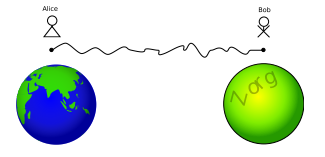
\includegraphics[scale=0.5]{images/ent.png}
        \end{center}
        
    \end{frame}
    \begin{frame}{Quantum Circuits}
        We present a series of quantum operations on qubits via a circuit which 
        each operation represents itself as a gate in our circuit
        \begin{block}{CNOT gate}
            \begin{center}
            \begin{quantikz}
                \lstick{x} & \ctrl{1} &
                \wire[l][1]["x"{above,pos=0.2}]{a} \\
                \lstick{y} & \targ{} & \rstick{x+y}
                \end{quantikz}
            \end{center}
        \end{block}
    \end{frame}
    \begin{frame}{Quantum Circuits}
        \begin{block}{Hadamard Gate}
            Hadarmand gate switches between $|0\rangle,|1\rangle$ and
            $|0\rangle+|1\rangle,|0\rangle-|1\rangle$ basis. The matrix for this operation
            is as follows: $
            \begin{bmatrix}
                \frac{1}{\sqrt{2}}&\frac{1}{\sqrt{2}}\\
                \frac{1}{\sqrt{2}}&-\frac{1}{\sqrt{2}}
            \end{bmatrix}$
            We represent this operation by following gate:\\
            \begin{center}
            \begin{quantikz}
                && \gate{H} &&
            \end{quantikz}
        \end{center}
            
        \end{block}
    \end{frame}
    \begin{frame}{Quantum Circuits}
        \begin{exampleblock}{Circuit example 1 }
            From what we learned we can introduce a circuit starting from unentangled states creating 
            entangled states\footnote{\url{https://en.wikipedia.org/wiki/Bell_state}}.\\
            \begin{center}
            \begin{quantikz}
                \lstick{\ket{0}} & \gate{H} & \ctrl{1} &&\\
                \lstick{\ket{0}} && \targ{} &&& \rstick{\ket{00} + \ket{11}}
            \end{quantikz}
        \end{center}
        \end{exampleblock}
    \end{frame}
    \begin{frame}{Quantum Circuits}
        \begin{exampleblock}{Circuit example 2 }
            The example from before about measurement between computations is as follows:\\
            \begin{center}
                \begin{quantikz}
                    \lstick{\ket{q}} & \gate{H} & \gate{H} & \meter{} & \rstick{NOT \ket{q}}\\
                    \lstick{\ket{q}} & \gate{H} & \meter{} & \gate{H} & \meter{} & \rstick{\ket{q} or NOT \ket{q}}
                \end{quantikz}
                % \begin{quantikz}
                %     \lstick{\ket{q}} & \gate{H} & \gate{H} & \meter{} & \rstick{NOT \ket{q}}
                    
                % \end{quantikz}
                
            \end{center}
        \end{exampleblock}
    \end{frame}
    \begin{frame}{Quantum Computation}
        \begin{itemize}
            \item What is the quantum computation model?
            \pause
            \item This question was answered in rigorous terms by Bernstein and Vzirani in a 70 page paper in 1993
            who defined a quantum Turing machine that could have the tape head and symbols and superpositions.
            \pause
            \item Independently, Andy Yao defined quantum circuits, which are computationally equivalent. This is
            what people use today because they are simpler.
        \end{itemize}
    \end{frame}
    \subsection{Subsection 1.2}
    % \begin{frame}[t]
    \begin{frame}
        This frame has an empty title and is aligned to top.
    \end{frame}
    
    % \begin{frame}[noframenumbering]{No frame numbering}
    \begin{frame}{No frame numbering}
        This frame is not numbered and is citing reference \cite{knuth74}.
    \end{frame}
    
    \begin{frame}{Typesetting and Math}
        The packages \texttt{fontenc} and \texttt{FiraSans}\footnote{\url{https://fonts.google.com/specimen/Fira+Sans}}\textsuperscript{,}\footnote{\url{http://mozilla.github.io/Fira/}} are used to properly set the main fonts.
        \vfill
        This theme provides styling commands to typeset \emph{emphasized}, \alert{alerted}, \textbf{bold}, \textcolor{example}{example text}, \dots
        \vfill
        \texttt{FiraSans} also provides support for mathematical symbols:
        \begin{align*}
            e^{i\pi} + 1 & = 0, \\
            \int_{-\infty}^\infty e^{-x^2}\,\mathrm{d}x & = \sqrt{\pi}.
        \end{align*}
    \end{frame}
    % \section{new section}
    % \begin{frame}

    % \end{frame}
    % \begin{frame}

    % \end{frame}
    % \begin{frame}

    % \end{frame}